\chapter{Methodology}
\label{ch:method}

This section details the methodology employed in this research. The approach is structured into several key components: data collection and processing, the modelling approach, and model explainability.

\section{Data}

\subsection{Database of East African Mesoscale Convective Systems (MCSs)}

In their paper, \cite{Hill2023} used a variant of the "simple-track" object tracking algorithm to identify and track \acrshortpl{mcs} over East Africa from infrared satellite imagery over 2014 to 2019 \citep{Stein2020}. The tracking algorithm identifies contiguous areas of cloud top brightness temperature (BT)\todo{acronym, especially to help table below?} below a threshold of \SI{233}{\kelvin}. The algorithm then tracks these areas over time based on their spatial overlap in consecutive images. The resulting database contains detailed information on the location, size, intensity, and duration of each MCS, as well as precipitation amounts derived from Global Precipitation Measurement (GPM) satellite imagery.

From this comprehensive storm database, a subset of approximately 30,000 was selected for analysis. Two criteria were used to filter for storms relevant to this study: 1) storms must be longer than 3 hours, and 2) all storm centroids must be located within the geographical bounds of (\degN{3} - \degN{15}, \degE{34} - \degE{52}). The 3-hour threshold was chosen because storms of this duration account for 92\% of MCS precipitation \citep{Hill2023}.

\subsection{ERA5 Data}

\acrfull{era5} is a reanalysis dataset produced by the \acrfull{ecmwf} which includes atmospheric, land, and oceanic climate variables from 1950 onwards \citep{Hersbach2020}. For this thesis, hourly data separated into yearly files was downloaded from the Copernicus Climate Change Service (C3S) Climate Data Store (CDS). The region for the data download was chosen to be slightly larger than the storm database region, covering (\degN{2} - \degN{16}, \degE{31} - \degE{53}). This buffer ensures that all storms are fully captured and to facilitate the calculation of gradients. The data was downloaded at a spatial resolution of \SI{0.25}{\degree} and includes the following meteorological variables relevant to storm development and propagation.

\begin{table}[ht]
    \centering
    \caption{ERA5 Data File Patterns, Descriptions, and Units}
    \label{tab:era5-file-patterns}
    \begin{tabular}{p{0.25\linewidth} p{0.45\linewidth} p{0.2\linewidth}}
        \toprule
        File Pattern & Description & Units/Notes \\
        \midrule
        \texttt{cape\_0\_*.nc} & Convective available potential energy & \unit{\joule\per\kilogram} \\
        \texttt{olr\_toa\_*.nc} & Top-of-atmosphere outgoing longwave flux (proxy for convection/clouds) & \unit{\watt\per\meter\squared} \\
        \texttt{prcp\_tot\_*.nc} & Thickness of rainfall amount (hourly accumulations) & \unit{\meter} \\
        \texttt{rhum\_*\_*.nc} & Relative humidity at 500, 750 and 900 \unit{\hecto\pascal} & \unit{\percent} (used for theta e calculations) \\
        \texttt{shum\_*\_*.nc} & Specific humidity at 200, 500, 850 \unit{\hecto\pascal} & \unit{\kilogram\per\kilogram} \\
        \texttt{skt\_sfc\_*.nc} & Surface temperature on land & \unit{\kelvin} \\
        \texttt{sst\_sfc\_*.nc} & Sea surface temperature & \unit{\kelvin} \\
        \texttt{swvl1\_d1\_*.nc} & Volumetric soil water layer 1 & \unit{\meter\cubed\per\meter\cubed} \\
        \texttt{swvl2\_d2\_*.nc} & Volumetric soil water layer 2 & \unit{\meter\cubed\per\meter\cubed} \\
        \texttt{ta\_*\_*.nc} & Air temperature at 500, 750 and 900 \unit{\hecto\pascal} & \unit{\kelvin} (used for theta e calculations) \\
        \texttt{tcwv\_tot\_*.nc} & Thickness of atmosphere mass content of water vapour & \unit{\kilogram\per\meter\squared} (total column water vapour) \\
        \texttt{thetae\_*\_*.nc} & Equivalent potential temperature at 500, 750 and 900 \unit{\hecto\pascal} & \unit{\kelvin} (dew point, LCL temperature, theta e via MetPy) \\
        \texttt{uwnd\_*\_*.nc} & Zonal wind at 200, 500 and 850 \unit{\hecto\pascal} & \unit{\meter\per\second} \\
        \texttt{vwnd\_*\_*.nc} & Meridional wind at 200, 500 and 850 \unit{\hecto\pascal} & \unit{\meter\per\second} \\
        \bottomrule
    \end{tabular}
\end{table}


\subsection{Feature Engineering and Selection}

Table \ref{tab:features} describes the X features used for this thesis and their respective units. These features were derived from the original storm database and \acrshort{era5} data through a series of processing steps. The features can be broadly categorised into three groups: storm-specific features, meteorological features, and geographical features. Features with the \texttt{mean\_} prefix are calculated over a 400 km radius square-area from the MCS centre and are instantaneous unless otherwise specified. Features with the \texttt{domain\_mean\_} prefix are calculated over the entire domain of the \acrshort{era5} and are also instantaneous unless otherwise specified. The \SI{400}{\km} radius was chosen to align with the original study by \cite{Hunt2024} and to capture the mesoscale environment surrounding each storm. The features without these prefixes are either directly sourced from the storm database or are derived from the \acrshort{era5} data at the grid points corresponding to the storm centroids.

{\small
\begin{longtable}{>{\raggedright\arraybackslash}p{0.25\linewidth} p{0.50\linewidth} >{\raggedright\arraybackslash}p{0.15\linewidth}}
    \caption{Features Used in the Study. Long feature names are wrapped for readability.} \\
    \label{tab:features} \\
    \toprule
    \textbf{Feature name} & \textbf{Description} & \textbf{Units} \\
    \midrule
    \endfirsthead

    \multicolumn{3}{c}%
    {{\bfseries \tablename\ \thetable{} -- continued from previous page}} \\
    \toprule
    \textbf{Feature name} & \textbf{Description} & \textbf{Units} \\
    \midrule
    \endhead

    \midrule \multicolumn{3}{r}{{Continued on next page}} \\
    \endfoot

    \bottomrule
    \endlastfoot

    \texttt{date\_angle} & Angle representation of current date within year & \unit{\degree} \\
    \texttt{eat\_hours} & Time step hour of day & \href{https://www.timeanddate.com/time/zones/eat}{Eastern Africa Time} (UTC+3) \\
    \texttt{storm\_total\_duration} & Total duration of MCS & \unit{\hour} \\
    \texttt{lon} & Longitude of MCS centre & \unit{\degree}E \\
    \texttt{lat} & Latitude of MCS centre & \unit{\degree}N \\
    \texttt{orography\_height} & Elevation of land surface at MCS centre & \unit{\meter} \\
    \texttt{anor} & Angle of sub-gridscale orography at MCS centre & radians from East \\
    \texttt{upslope\_bearing} & Compass bearing of upslope direction at MCS centre & \unit{\degree} from  N \\
    \texttt{slope\_angle} & Angle of slope at MCS centre & \unit{\degree} \\
    \texttt{over\_land} & Flag for MCS centre (True if MCS centre is over land, else False) & \texttt{boolean} \\
    \texttt{acc\_land\_time} & Accumulated time where \texttt{over\_land}=True & \unit{\hour} \\
    \texttt{storm\_total\_land\_time} & Final value of \texttt{acc\_land\_time} for MCS & \unit{\hour} \\
    \texttt{mean\_land\_frac} & Fraction of area within 400 km that is over land & ratio ($[0,1]$) \\
    \texttt{zonal\_speed} & $x$-component of MCS centre propagation vector & \unit{\km\per\hour} \\
    \texttt{meridional\_speed} & $y$-component of MCS centre propagation vector & \unit{\km\per\hour} \\
    \texttt{area} & Area of the MCS & \unit{\km\squared} \\
    \texttt{storm\_max\_area} & Max value of \texttt{area} over MCS & \unit{\km\squared} \\
    \texttt{bearing\_from\_prev} & Compass bearing from previous observation & \unit{\degree} from  N \\
    \texttt{bearing\_to\_next} & Compass bearing to next observation & \unit{\degree} from  N \\
    \texttt{distance\_from\_prev} & Distance traversed from previous observation & \unit{\km} \\
    \texttt{distance\_to\_next} & Distance to next observation & \unit{\km} \\
    \texttt{distance\_traversed} & Cumulative sum of \texttt{distance\_from\_prev} & \unit{\km} \\
    \texttt{storm\_bearing} & Compass bearing from first to last MCS centre & \unit{\degree} from  N \\
    \texttt{storm\_distance \_traversed} & Total cumulative distance traversed by MCS centre & \unit{\km} \\
    \texttt{storm\_straight \_line\_distance} & Distance from first to last MCS centre & \unit{\km} \\
    \texttt{mean\_skt} & Surface temperature & \unit{\kelvin} \\
    \texttt{mean\_land\_skt} & Land surface temperature (NaN if entire area is ocean) & \unit{\kelvin} \\
    \texttt{mean\_sst} & Sea surface temperature (NaN if entire area is land) & \unit{\kelvin} \\
    \texttt{mean\_swvl1} & Volumetric soil moisture in the top layer ($<$7 cm; NaN over ocean) & \unit{\meter\cubed\per\meter\cubed} \\
    \texttt{mean\_swvl2} & Volumetric soil moisture in the second layer (7--28 cm; NaN over ocean) & \unit{\meter\cubed\per\meter\cubed} \\
    \texttt{mean\_u850} & \SI{850}{\hecto\pascal} zonal wind & \unit{\meter\per\second} \\
    \texttt{mean\_u500} & \SI{500}{\hecto\pascal} zonal wind & \unit{\meter\per\second} \\
    \texttt{mean\_u200} & \SI{200}{\hecto\pascal} zonal wind & \unit{\meter\per\second} \\
    \texttt{mean\_v850} & \SI{850}{\hecto\pascal} meridional wind & \unit{\meter\per\second} \\
    \texttt{mean\_v500} & \SI{500}{\hecto\pascal} meridional wind & \unit{\meter\per\second} \\
    \texttt{mean\_v200} & \SI{200}{\hecto\pascal} meridional wind & \unit{\meter\per\second} \\
    \texttt{domain\_mean\_u500} & Mean \SI{500}{\hecto\pascal} zonal wind over the entire domain of ERA5 data & \unit{\meter\per\second} \\
    \texttt{mean\_u\_shear\_850\_500} & Shear of zonal wind from \SI{850}{\hecto\pascal} to \SI{500}{\hecto\pascal} & \unit{\meter\per\second} \\
    \texttt{mean\_v\_shear\_850\_500} & Shear of meridional wind from \SI{850}{\hecto\pascal} to \SI{500}{\hecto\pascal} & \unit{\meter\per\second} \\
    \texttt{mean\_u\_shear\_850\_200} & Shear of zonal wind from \SI{850}{\hecto\pascal} to \SI{200}{\hecto\pascal} & \unit{\meter\per\second} \\
    \texttt{mean\_v\_shear\_850\_200} & Shear of meridional wind from \SI{850}{\hecto\pascal} to \SI{200}{\hecto\pascal} & \unit{\meter\per\second} \\
    \texttt{wind\_direction\_850} & Compass bearing from which the \SI{850}{\hecto\pascal} wind vector at MCS centre originates & \unit{\degree} from  N \\
    \texttt{wind\_angle\_upslope} & Angle of \texttt{wind\_direction\_850} relative to \texttt{upslope\_bearing} (wind is going upslope: \ang{0}, downslope: \ang{180}, cross-slope: \ang{90}, \ang{270}) & \unit{\degree} from \texttt{upslope\_bearing} \\
    \texttt{mean\_tcwv} & Total column water vapour (TCWV) & \unit{\kilogram\per\meter\squared} \\
    \texttt{domain\_mean\_tcwv} & Mean TCWV over the entire domain of ERA5 data & \unit{\kilogram\per\meter\squared} \\
    \texttt{mean\_q\_850} & \SI{850}{\hecto\pascal} specific humidity & \unit{\kilogram\per\kilogram} \\
    \texttt{mean\_q\_500} & \SI{500}{\hecto\pascal} specific humidity & \unit{\kilogram\per\kilogram} \\
    \texttt{mean\_q\_200} & \SI{200}{\hecto\pascal} specific humidity & \unit{\kilogram\per\kilogram} \\
    \texttt{mean\_cape} & Convective available potential energy (CAPE) & \unit{\joule\per\kilogram} \\
    \texttt{domain\_mean\_cape} & Mean CAPE over the entire domain of ERA5 data & \unit{\joule\per\kilogram} \\
    \texttt{olr\_90} & 90th percentile of negative outgoing longwave radiation (OLR) within 400 km & \unit{\watt\per\square\meter} \\
    \texttt{olr\_75} & 75th percentile of negative OLR within 400 km & \unit{\watt\per\square\meter} \\
    \texttt{olr\_50} & 50th percentile of negative OLR within 400 km & \unit{\watt\per\square\meter} \\
    \texttt{mean\_prcp\_400} & Precipitation over the next 6 hr & \unit{\milli\meter} \\
    \texttt{min\_bt} & Minimum cloudtop brightness within MCS area & \unit{\kelvin} \\
    \texttt{dmin\_bt\_dt} & Rate of change of \texttt{min\_bt} & \unit{\kelvin\per\hour} \\
    \texttt{mean\_bt} & Mean cloudtop brightness within MCS area & \unit{\kelvin} \\
    \texttt{dmean\_bt\_dt} & Rate of change of \texttt{mean\_bt} & \unit{\kelvin\per\hour} \\
    \texttt{storm\_min\_bt} & Minimum value of \texttt{min\_bt} reached over MCS lifetime & \unit{\kelvin} \\
    \texttt{storm\_min\_bt\_reached} & False if \texttt{storm\_min\_bt} has not been reached yet, else True & \texttt{boolean} \\
    \texttt{mjo\_phase} & Phase of Madden--Julian oscillation (MJO) & $[1, 8] \cap \mathbb{Z}$ \\
    \texttt{mjo\_amplitude} & Amplitude of MJO & - \\
\end{longtable}
}

The following highly correlated features were identified and removed to prevent redundancy and reduce the risk of multicollinearity, which can negatively impact model interpretability and performance.
\begin{itemize}
    \item \texttt{mean\_swvl1} and \texttt{mean\_swvl2} have a Pearson correlation coefficient of 0.94 and thus \texttt{mean\_swvl2} was removed.
    \item \texttt{olr\_90}, \texttt{olr\_75}, \texttt{olr\_50} were all correlated with coefficients above 0.8, so only \texttt{olr\_90} was retained.
\end{itemize}
Additionally, measures were implemented to prevent data leakage, including the careful exclusion of features that are directly related to the target variable or contain information from future time steps that would not be available at prediction time. These steps help ensure that the model learns meaningful relationships from the data and that its predictive performance is not artificially inflated by access to information that would not be present in a real-world forecasting scenario. A full correlation heatmap is available in Appendix \insertref{app:correlation-heatmap}.

\section{Modelling Approach}

The following section describes the \acrshort{ml} approach taken to predict storm intensification and propagation. As all predictands are continuous variables and the input features can be directly associated with the target storm characteristics, this \acrshort{ml} task is classified as supervised regression as opposed to unsupervised learning, where the target variables are not known, or classification, where the goal is to predict discrete labels.

\subsection{XGBoost}

In this thesis, \acrfull{xgb} is the modelling framework employed for this supervised regression task. In part, the decision to use \acrshort{xgb} corresponds with faithfully reproducing the methodology of \cite{Hunt2024}. However, their choice is justified by the advantages that the approach presents. \acrshort{xgb} is a decision-tree based model leveraging an efficient and scalable implementation of gradient boosting \citep{Chen2016}. Gradient boosting, an extension of \gls{ensemblelearning}, iteratively trains weak learners, in this case decision trees, on the residual errors of the previous learners. This process allows the model to focus on the most challenging examples to improve overall performance while also preventing overfitting, especially when compared to one, highly complex decision tree model \citep{Friedman2001}. Yet, since the model retains its underlying structure of decision trees, it remains directly interpretable through techniques like feature importance. Generally, feature importance is a global model-agnostic \acrshort{xai} method that quantifies the contribution of each feature to the model's predictions by measuring the change in the model's performance when the feature is permuted \citep{Musolf2022}. In decision-tree based models, the nature of the trees themselves can be exploited to more efficiently calculate importance. Typically, this is based on metrics like the frequency with which a feature is used for splitting, the average gain in accuracy from splits involving that feature, or the total reduction in impurity attributed to that feature across all trees in the ensemble \citep{Louppe2013}. Although not used in this thesis, the inherent interpretability of \acrshort{xgb} through feature importance analysis aligns with the goals of this research.

\subsection{Hyperparameter Tuning}

\acrshort{xgb} provides a myriad of hyperparameters that can be adjusted to optimise model performance. These include parameters controlling the learning rate, tree depth, number of trees, and regularisation terms, among others. The choice of hyperparameters can significantly impact the model's ability to generalise to unseen data. Therefore, a systematic approach to hyperparameter tuning is essential. 

In this thesis, hyperparameter tuning is conducted using \acrfull{wandb}, a popular web-based tool for tracking and visualising \acrshort{ml} experiments \citep{Biewald2020}. Specifically, Bayesian optimisation is employed to efficiently explore the hyperparameter space and identify optimal configurations. Bayesian optimisation is particularly well-suited for this task as it builds a probabilistic model of the cost function and uses it to select the most promising hyperparameters to evaluate next \citep{Mockus1994,Shahriari2016}\todo{better desc/wording}. This approach balances exploration and exploitation, allowing for a more efficient search compared to grid or random search methods. 

For regression tasks, many metrics can be used to evaluate model performance. In this thesis, \acrfull{rmse} is used because, by square rooting the mean of the squared errors, it provides a measure of error in the same units as the original predictions and is therefore more interpretable. Thus, Bayesian optimisation is set to minimise the validation \acrshort{rmse} during hyperparameter tuning. By default, \acrshort{wandb} sweeps will continue until manually stopped unless a maximum trial count is provided. For this thesis, a maximum trial count of 20 is used. \todo{this value might change}

Additionally, cross-validation is utilised during training on each trial to ensure that the model's performance is robust and not overly dependent on a specific subset of the data. Specifically, the dataset is first split into a training set and a test set to ensure that some data remains completely unseen throughout the training process. Then, within the training set, k-fold cross-validation is applied, where the dataset is divided into k subsets and the model is trained and validated k times, each time using a different subset as the validation set and the remaining subsets for training. Once all folds are complete, the best performing model is chosen as the result of the trial. This method provides a more reliable estimate of model performance on the given hyperparameters \citep{Lopez2023,Singh2021}\todo{better desc/wording}.

The specific hyperparameters tuned and the corresponding values or distributions used for the sweep are included in Table \ref{tab:wandb-sweep-config}. The remaining hyperparameters were kept at their default values as defined in the \acrshort{xgb} Python implementation \insertref{need a link to xgb docs here similar to Hunt2024?}.

\begin{table}[!ht]
    \centering
    \caption{\acrshort{wandb} Sweep Configuration for \acrshort{xgb} Hyperparameter Tuning. The names in this table refer to the hyperparameter names for the Scikit-Learn wrapper interface for \acrshort{xgb}. A full description of each hyperparameter can be found in the \href{https://xgboost.readthedocs.io/en/stable/python/python_api.html\#module-xgboost.sklearn}{XGBoost documentation}.}
    \label{tab:wandb-sweep-config}
    \begin{tabular}{llr}     
        \toprule
        \textbf{Hyperparameter} & \textbf{Values / Distribution} \\ 
        \midrule
        Gamma ($\gamma$) & Uniform[0, 5] \\
        Regularisation Alpha ($\alpha$) & Uniform[0, 5] \\
        Regularisation Lambda ($\lambda$) & Uniform[0, 5] \\
        Column Subsample by Tree & Uniform[0, 1.0] \\
        Learning Rate & Uniform[0, 1.0] \\
        Max Depth & \{3, 6, 9, 12\} \\
        Number of Estimators & \{60, 120, 180\} \\
        \bottomrule
    \end{tabular}
\end{table}

Once the sweeps are complete, the best models from each sweep are evaluated on the held-out test set to provide an unbiased estimate of their performance. The test \acrshort{rmse} values are first compared with the standard deviation of the target variable in the test set to assess whether the model has successfully captured novel relationships beyond just the underlying distribution of the target. They are then compared across different models and feature sets to assess relative performance. Furthermore, test \acrshort{rmse} over the dataset region and time period is analysed to identify any spatial or temporal patterns in model performance. \todo{if no time, this is for future work section}

\section{Model Explainability}
\todo{copied from background; will need to be adapted}

\acrfull{xai} is an emerging field focused on developing methods and techniques to make the decision-making processes of \acrshort{ml} solutions more transparent and interpretable. Approaches in this field take a variety of forms, including inherently interpretable models and post-hoc explanation methods. A summary of \acrshort{xai} taxonomy is given in Figure \ref{fig:xai-taxonomy}.

\begin{figure}[ht]
    \centering
    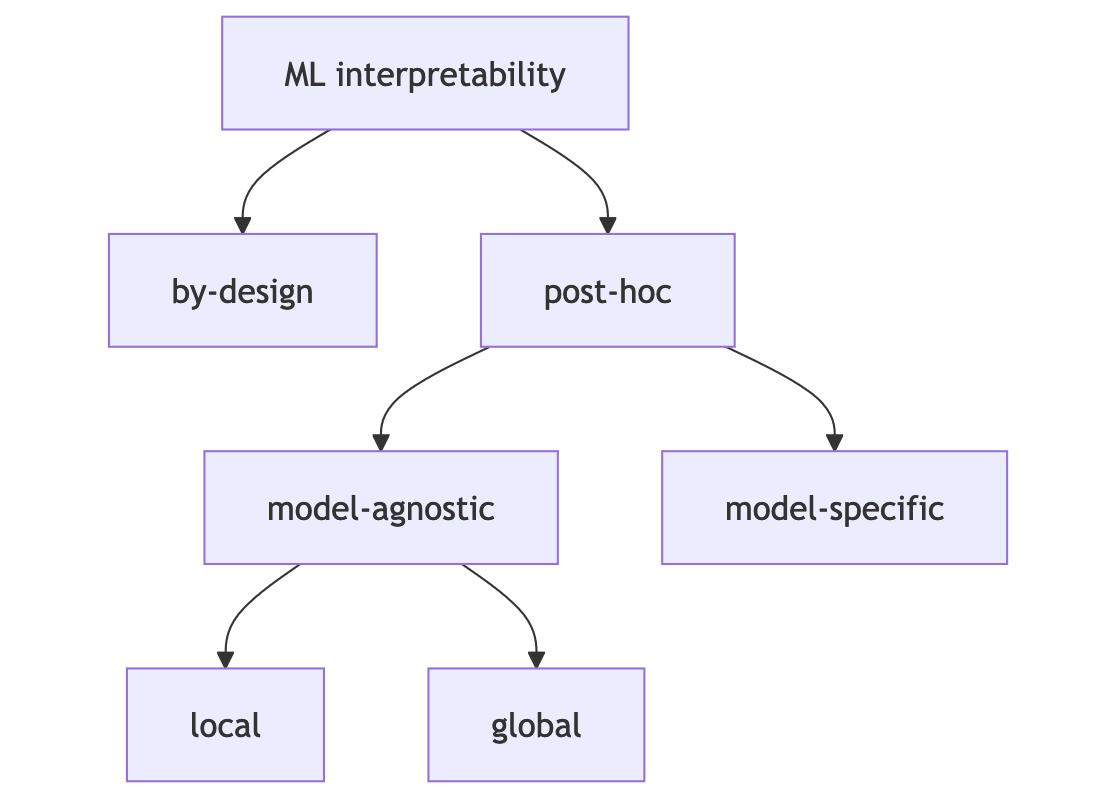
\includegraphics[width=0.8\textwidth]{../figures/static/xai-taxonomy.jpg}
    \caption{\acrshort{xai} Taxonomy \citep{Molnar2025}}
    \label{fig:xai-taxonomy}
\end{figure}

Inherently interpretable models are designed to be transparent by construction, often using simpler architectures or feature-based approaches that allow for direct interpretation of the relationship between inputs and outputs. Examples include linear regression, decision trees, and rule-based systems. A clear disadvantage is that these simpler models may sacrifice some predictive performance compared to more complex ones like \acrfull{dnn}. \acrshort{piml} could also be considered a part of this landscape, as it aims to integrate existing physical knowledge into architectures and training processes to enhance forecast accuracy and credibility. Post-hoc explanation methods, on the other hand, are applied to models after training to partially interpret their behaviour. Model-specific post-hoc methods leverage the learned structure of the model. Feature importance, as mentioned above, serves as a illustrative example, where the decision-tree model structure is integrated directly into the explanation algorithm. Notably for this research, model-agnostic methods are predominantly designed to make no assumptions about a model's underlying architecture. These methods can then be broadly categorised into local and global explanations. Local explanations focus on providing insights into model behaviour around a given input. In contrast, global explanations aim to provide an overall understanding of the model's behaviour for any input. For local explanations, counterfactual analysis has gained traction, especially for classification tasks, where the model's local decision boundary can be more interactively explored through slight perturbations of the a given input \citep{Mothilal2019}. \acrfull{shap} is both applicable for local and global explanations and will be used extensively throughout this research. As such, a brief overview of the approach follows.

\subsection{Shapley Additive Explanations}

After its popularisation via \cite{Lundberg2017} and the accompanying \texttt{shap} \texttt{python} library, \acrfull{shap} has emerged as one of the most prominent frameworks for post-hoc explainability. This is achieved through the application of coalitional game theory where the algorithm approximates a fair distribution of "payout", in this case a fraction of the model's prediction, among the input features based on their individual contributions to the prediction \citep{Shapley1953}. Formally, the Shapley value for a feature is calculated via the average marginal contribution of that feature across all possible coalitions of features weighted by the probability of the coalition, where a coalition is a subset of features, and the marginal contribution of a feature to a coalition is the difference in the model's prediction when that feature is included versus when it is excluded. This process ensures that each feature's contribution is fairly evaluated by accounting for its interactions with other features. The result is a set of Shapley values for each feature and model output, which can then be used to interpret the model's predictions locally, by highlighting the most influential features for a single output, or globally, by aggregating the Shapley values across multiple predictions to identify overall feature importance.

In practice, this algorithm experiences a \gls{combinatorialexplosion} as features increase, thus, various approximations and optimisations have been developed to make it feasible for larger datasets. For example, \cite{Lundberg2017} present a kernel-based method which operates on the assumption that not all coalitions are equally important in quantifying a features marginal contribution. The application of Shapley values for explaining \acrshort{ml} models was first proposed by \cite{trumbelj2011}, but \cite{Lundberg2017} key contribution was the introduction of an additive feature attribution model, which allows for efficient approximation using a linear model. This approach assumes that the prediction can be expressed as a sum of the feature contributions, making it easier to interpret and visualise. The \texttt{shap} library implements both model-specific and agnostic methods using this framework and provides various tools for visualising Shapley values and their impact on individual predictions and overall model performance.

In this thesis, \acrshort{shap} is primarily used to as a global explanation method. The goal is to identify the most important features driving model predictions across the entire dataset. This is achieved by calculating the mean absolute Shapley value for each feature across all predictions, which provides a measure of overall feature importance. The results are visualised using summary plots to simultaneously convey both the magnitude and direction of each feature's impact on the model's predictions. In addition, the spatial and temporal distribution of feature importance will be analysed to identify any regional or temporal patterns in the model's behaviour. Potential candidate features will be identified by correlating Shapley values with observation coordinates and timestamps. Top candidates will be analysed by mapping their Shapley values across the study region and time period. Such analyses are aimed to uncover which features are most dependent on location and time, potentially revealing underlying physical relationships captured by the model.

\section{Experimental Setup}

The experimental setup is designed to systematically evaluate the performance of the proposed models under different conditions and feature sets. The experiments are divided into two groups: storm aggregate characteristic prediction tasks and immediate characteristics at observation prediction tasks. Storm aggregate tasks involve predicting characteristics that summarise the entire lifecycle of a storm with the aim of understanding its overall behaviour and impact. In contrast, immediate characteristic tasks focus on predicting properties at each observation time step, such as the 6-hour mean precipitation and rate of intensification. These tasks require a more granular understanding of the storm's evolution and are more applicable to real-time forecasting applications.

For all experiments, two models were trained on two different feature sets: all available features and only ERA5 meteorological features. This approach allows for a comparison of model performance when utilising a focused subset of variables. While it is likely that storm genesis location and orography over the track will play a major role, it is possible that those features could confound the effects of other environmental factors like soil moisture or skin temperature. Thus, through this setup, we ensure that one model is exclusively learning from the meteorological conditions. If model performance differs significantly, this would imply that the geographic, topological, or temporal features contain unique information not captured by the meteorological features. Through a comparison of relative feature importance of the meteorological features, we can also gain insights into their interaction with the other features. In addition, for the storm aggregate prediction tasks, two additional models were trained using only the first observation of each storm, again comparing all features versus only ERA5 features. This aspect of the setup aims to evaluate the predictive power of initial storm observations.

The experiments conducted are summarised in Table \ref{tab:experimental-setup}.

{\small
\begin{longtable}{>{\raggedright\arraybackslash}p{0.27\linewidth} p{0.43\linewidth} >{\raggedright\arraybackslash}p{0.20\linewidth}}
    \caption{Experiments Summary. Long experiment names are wrapped for readability.} \\
    \label{tab:experimental-setup} \\
    \toprule
    \textbf{Experiment alias} & \textbf{Description} & \textbf{Predictand} \\
    \midrule
    \endfirsthead

    \multicolumn{3}{c}%
    {{\bfseries \tablename\ \thetable{} -- continued from previous page}} \\
    \toprule
    \textbf{Experiment alias} & \textbf{Description} & \textbf{Predictand} \\
    \midrule
    \endhead

    \midrule \multicolumn{3}{r}{{Continued on next page}} \\
    \endfoot

    \bottomrule
    \endlastfoot

    \multicolumn{3}{c}{\textit{Storm Aggregate Prediction Tasks}} \\
    \midrule
    \texttt{storm\_max\_intensity\_all} & Predict storm minimum BT using all features and all observations & \texttt{storm\_min\_bt} \\
    \texttt{storm\_max\_intensity\_all \_first\_points} & Predict storm minimum BT using all features and first observation only & \texttt{storm\_min\_bt} \\
    \texttt{storm\_max\_intensity\_era5} & Predict storm minimum BT using ERA5 features and all observations & \texttt{storm\_min\_bt} \\
    \texttt{storm\_max\_intensity\_era5 \_first\_points} & Predict storm minimum BT using ERA5 features and first observation only & \texttt{storm\_min\_bt} \\
    \texttt{storm\_direction\_all} & Predict storm bearing using all features and all observations & \texttt{storm\_bearing} \\
    \texttt{storm\_direction\_all \_first\_points} & Predict storm bearing using all features and first observation only & \texttt{storm\_bearing} \\
    \texttt{storm\_direction\_era5} & Predict storm bearing using ERA5 features and all observations & \texttt{storm\_bearing} \\
    \texttt{storm\_direction\_era5 \_first\_points} & Predict storm bearing using ERA5 features and first observation only & \texttt{storm\_bearing} \\
    \midrule
    \multicolumn{3}{c}{\textit{Immediate Characteristic Prediction Tasks}} \\
    \midrule
    \texttt{obs\_intensification\_all} & Predict rate of change of minimum BT using all features & \texttt{dmin\_bt\_dt} \\
    \texttt{obs\_intensification\_era5} & Predict rate of change of minimum BT using ERA5 features & \texttt{dmin\_bt\_dt} \\
    \texttt{obs\_next\_direction\_all} & Predict bearing to next observation using all features & \texttt{bearing\_to\_next} \\
    \texttt{obs\_next\_direction\_era5} & Predict bearing to next observation using ERA5 features & \texttt{bearing\_to\_next} \\
    \texttt{obs\_next\_distance\_all} & Predict distance to next observation using all features & \texttt{distance\_to\_next} \\
    \texttt{obs\_next\_distance\_era5} & Predict distance to next observation using ERA5 features & \texttt{distance\_to\_next} \\
    \texttt{obs\_precipitation\_all} & Predict 6-hour mean precipitation using all features & \texttt{mean\_prcp\_400} \\
    \texttt{obs\_precipitation\_era5} & Predict 6-hour mean precipitation using ERA5 features & \texttt{mean\_prcp\_400} \\
\end{longtable}
}